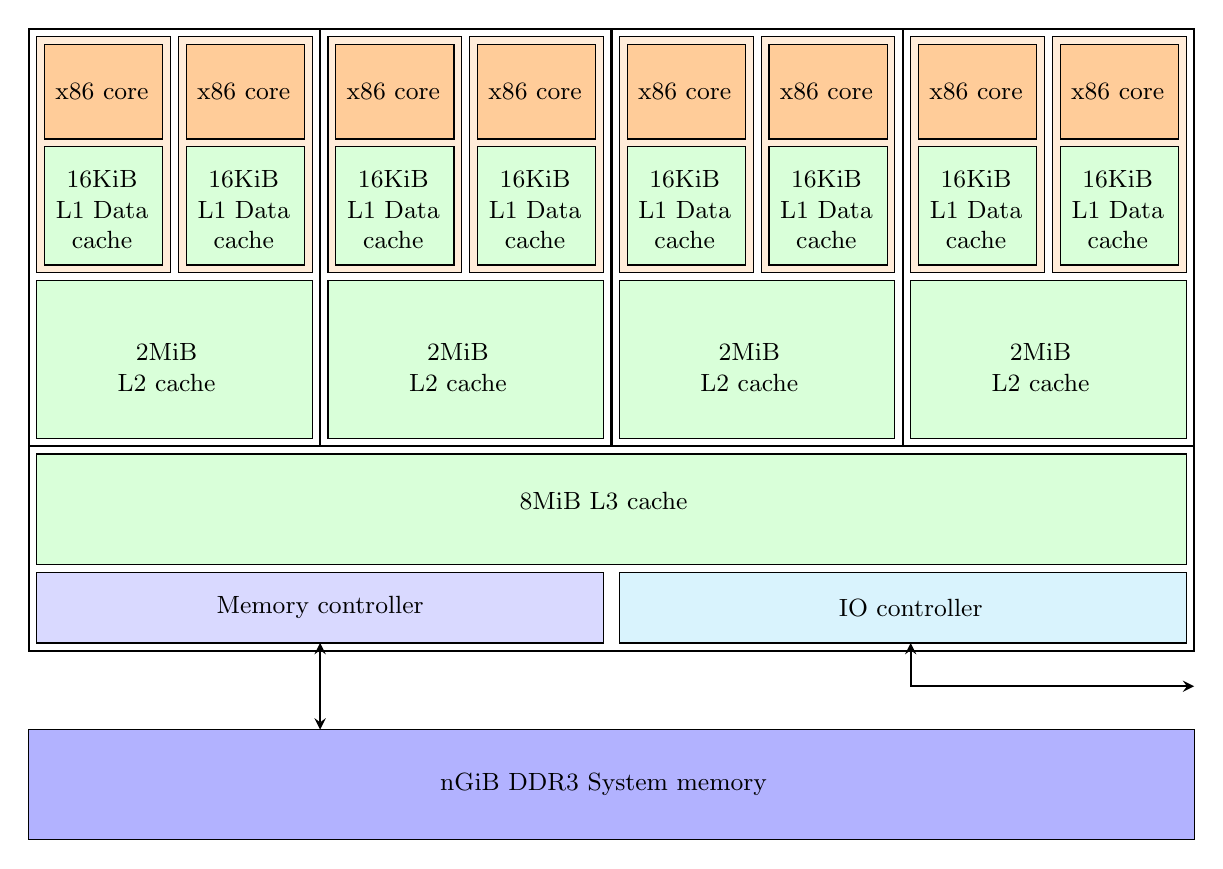
\begin{tikzpicture}[>=stealth]
\draw[thick] (0,0) rectangle ++(14.8, -2.6);
\foreach \x in {0,3.7,7.4,11.1}
{
  \draw[thick] (\x,0) rectangle ++(3.7,5.3);
  \draw[fill=green!15] (\x+0.1,0.1) rectangle ++(3.5,2);
  \draw node[text width=2cm,font=\small, align=center] at (\x+1.75 ,1) {2MiB\\L2 cache};
  \foreach \y in {0,1.8}
  {
    \draw[fill=orange!15] (\x+\y+0.1, 2.2) rectangle ++(1.7,3);
    \draw[fill=green!15] (\x+\y+0.2, 2.3) rectangle ++(1.5,1.5);
    \draw node[text width=1.5cm,font=\small, align=center] at (\x+\y+0.2+0.73, 3.0) {16KiB L1 Data cache};

    \draw[fill=orange!40] (\x+\y+0.2, 3.9) rectangle ++(1.5,1.2);
    \draw node[text width=1.2cm,font=\small, align=center] at (\x+\y+0.2+0.73, 4.5) {x86 core};
  }
}
\draw[fill=green!15] (0.1, -1.5) rectangle ++(14.6, 1.4);
\draw node[text width=3cm,font=\small, align=center] at (7.3,-0.7) {8MiB L3 cache};

\draw[fill=blue!15] (0.1, -2.5) rectangle ++(7.2, 0.9);
\draw node[text width=4cm,font=\small, align=center] at (3.7,-2.05) {Memory controller};

\draw[fill=cyan!15] (7.5, -2.5) rectangle ++(7.2, 0.9);
\draw node[text width=4cm,font=\small, align=center] at (7.5+3.7,-2.05) {IO controller};

\draw[fill=blue!30] (0, -5) rectangle ++(14.8, 1.4);
\draw node[text width=5.2cm,font=\small, align=center] at (7.3,-4.3) {nGiB DDR3 System memory};

\draw[thick, <->] (3.7,-2.5) -- (3.7, -3.6);

\draw[thick, <->] (7.5+3.7,-2.5) -- (7.5+3.7, -3.05) -- (14.8, -3.05);

\end{tikzpicture}